\chapter{GRAMS Experiment Apparatus}
\label{chap:GRAMS}

As mentioned in introduction Section.~\ref{chap:intro:GRAMS}, GRAMS is a novel project that can simultaneously target both astrophysical observations with MeV gamma rays and an indirect dark matter search with antimatter detection \cite{aramaki2020dual}. For GRAMS timeline showing in Fig.~\ref{fig:timeline}, we have finished engineer flight eGRAMS, antiproton beam test T98, and currently working on a prototype flight pGRAMS using a $ 30\ cm \times 30\ cm \times 30\ cm $ miniGRAMS detector with segmentation to measure MeV gamma-ray events and cosmic charged particle events.


\section{Liquid argon time projection chamber detector}
\label{chap:GRAMS:detectors}
The Liquid Argon Time Projection Chamber (LArTPC) is a powerful detection technology that has evolved significantly since its inception. The concept was first proposed by Nygren in 1974 as a method for precision tracking and calorimetry in particle physics experiments \cite{NYGREN201822}. Early implementations demonstrated the technology's ability to provide excellent spatial resolution and energy reconstruction capabilities through ionization charge collection in liquid argon medium.

Over the decades, LArTPC technology has matured through numerous experiments, including the pioneering work at Fermilab and subsequent large-scale implementations. The technology gained prominence with experiments such as MicroBooNE, which validated LArTPC performance for neutrino detection \cite{MicroBooNE:2007ivj}. More recently, the Deep Underground Neutrino Experiment (DUNE) has adopted LArTPC as its primary detection technology for next-generation physics research. The key advantages of LArTPC detectors include exceptional spatial resolution (sub-millimeter scale), excellent calorimetric capabilities for energy measurement, and the ability to reconstruct complex particle interaction topologies \cite{FALCONE2022167217}. These characteristics make LArTPC technology particularly suitable for both astrophysical gamma-ray observations and rare event searches, as demonstrated by the GRAMS mission.

The LArTPC operates on the principle of ionization charge collection in liquid argon. When a charged particle traverses the detector volume, it ionizes argon atoms along its path, creating electron-ion pairs. An applied electric field drifts the free electrons toward the anode (charge readout plane), while the ions drift toward the cathode. The charge collected at the anode is proportional to the energy deposited by the particle, enabling precise energy measurement and calorimetry.

Scintillation light is produced during the ionization process and is detected by photomultiplier tubes (PMTs) or silicon photomultipliers (SiPMs) positioned at the cathode. This light signal provides the initial trigger and timing reference (T$_0$) for the event. The time difference between the scintillation light detection and the charge signal arrival determines the drift time, which directly translates to the vertical (Z) coordinate of the interaction from electron drift speed calculation. Combined with the two-dimensional information from the charge readout grid, the full three-dimensional position of the event can be reconstructed with sub-millimeter precision.

The pixel-grid or mesh style structure of the charge readout allows determination of the horizontal (X and Y) coordinates by identifying which readout channels recorded a signal, details see Section.~\ref{chap:GRAMS:pGRAMS:RandD:detector}. This combination of spatial information from multiple detection mechanisms enables comprehensive event reconstruction and particle identification, making LArTPC ideal for complex interaction topologies.

\begin{table}
\centering
%\renewcommand{\arraystretch}{1.2} % Increase row spacing
\begin{tabularx}{\linewidth}{l >{\raggedleft\arraybackslash}X}
\toprule
\textbf{Property} & \textbf{Value} \\
\midrule
Normal boiling point (NBP) & 87.303(2) K \\
Normal freezing point & 83.8(3) K \\
Density at NBP & 1.396(1) g/ml \\
Heat of vaporization & 161.14 kJ/kg \\
Heat capacity & 1.117 kJ/kg/K \\
Mean energy per ionization $w$ & 23.6(3) eV/pair \\
Fano factor & 0.107 \\
Molière radius $R_M$ & 10.0 cm \\
Radiation length $X_0$ & 14.0 cm \\
Critical energy $E_c$ & 30.5 MeV \\
Nuclear interaction length $\lambda_I$ & 85.7 cm \\
Minimum ionization loss $dE/dx_{\text{min}}$ & 2.12 MeV/cm \\
\bottomrule
\end{tabularx}
\caption{Main physical properties of liquid argon under 1 atm pressure. See \cite{lar_properties, LI2016160, Thorn_lar_properties}. Detailed argon properties could be found in table.~\ref{tab:argon}}
\label{tab:main_LAr_properties}
\end{table}

\section{GRAMS Detection Concept}
\label{chap:GRAMS:concept}
This thesis focus mainly on the indirect \ac{DM} serarches with antinuclei, as the MeV gamma-ray detection concept has been well explained in \cite{aramaki2020dual}, I will give a brief introduction here in Section.~\ref{chap:GRAMS:concept:gamma}. Indirect \ac{DM} searches with antinuclei detection concept will be explained in Section.~\ref{chap:GRAMS:concept:antimatter} and further analysis will be shown in Section.~\ref{chap:GRAMSresult:antihelium-3}.

\subsection{GRAMS Detection Concept for MeV Gamma-rays}
\label{chap:GRAMS:concept:gamma}

As Fig.~\ref{fig:GRAMS_Concept} showed, Particles entering the LArTPC detector excite and ionize argon atoms, producing scintillation light and ionization electrons. The scintillation light measured by \ac{SiPM}s is used for triggering and timing of the event. The ionization electrons drift in an applied electric field and are collected at anode planes with a $\sim 2.8$~mm pitch of strips. The signals induced on the anode provide the $x$ and $y$ coordinates of the event, while the drift time of the ionization electrons gives the $z$ position. The ability to reconstruct three-dimensional space points without a multi-layered design is one of the key advantages for GRAMS compared to other gamma-ray detectors with semiconductors or scintillation crystals.

To reduce the coincident background during the finite collection time of the ionization signal, the LArTPC drift volume is segmented into ``cells'' with PTFE sheets. The detector can be further upgraded for a future satellite mission that focuses on the gamma-ray observations. The overall instrumental size can be $\sim 1.5$~m $\times 1.5$~m $\times 30$~cm without the outer scintillator layer while using a fine pitch ($\sim 0.2$~mm) of anode tile to track Compton-scattered electrons. We can also add a calorimeter around the detector, such as a \ac{CZT} detector, similar to a future satellite mission e-ASTROGAM~\cite{10.1007/s10686-017-9533-6}, in order to measure the escaping gamma rays and pair-produced electrons and positrons. We are currently working towards the development of a prototype detector, and the details of the readout electronics and the telemetry system will be determined in the future.

The MeV gamma-ray survey requires accurate reconstruction of the photon energy and direction. For energies above the electron-positron pair-production threshold ($E > 2m_e c^2$), GRAMS uses the precise tracking capability of the LArTPC to reconstruct the momentum of the electron-positron pair to determine the incident gamma ray. At lower energies, where gamma rays preferably undergo Compton scattering and photo-absorption, GRAMS relies on accurately determining the position and energy of the Compton electron and photo-absorption.

\begin{figure}
    \centering
    \includegraphics[width=1\linewidth]{fig/GRAMS_Compton_rings.png}
    \caption{Compton-scattering events in GRAMS. Three or more Compton “Event Circles” provide the direction of the gamma-ray source \cite{aramaki2020dual}.}
    \label{fig:GRAMS_compton_ring}
\end{figure}

Reconstruction of the incident gamma-ray energy $E$ and cone angle $\theta$ can be estimated by the Compton equation \cite{KAMAE1987254,DOGAN1990501}. A gamma ray may undergo a number of Compton scatterings before being photo-absorbed or even escape the sensitive volume of the detector (see Fig.~\ref{fig:GRAMS_compton_ring}). For one or two Compton scatterings followed by photo-absorption, the energy and cone angle can be calculated as below:

\begin{align}
E &= E_1 + E_2 + E_3 \\
\cos\theta &= 1 - m_e c^2 \left( \frac{1}{E_2 + E_3} - \frac{1}{E_1 + E_2 + E_3} \right) \\
\cos\theta' &= 1 - m_e c^2 \left( \frac{1}{E_3} - \frac{1}{E_2 + E_3} \right)
\end{align}

where $m_e$ is the electron mass, $E_1$, $E_2$, and $E_3$ are the deposited energies by the Compton scatterings and photo-absorption, and $\theta$ and $\theta'$ are the first and the second Compton scattering angles. For a single Compton scattering followed by a photo-absorption, the above simplifies since there is no $\theta'$ and $E_2 = 0$.

For an event with three or more Compton scatterings, the angle and energy can be reconstructed as below:

\begin{align}
E &= E_1 + E_2 + E'_3 \\
\cos\theta &= 1 - m_e c^2 \left( \frac{1}{E_2 + E'_3} - \frac{1}{E_1 + E_2 + E'_3} \right) \\
E'_3 &= -\frac{E_2}{2} + \sqrt{ \frac{E_2^2}{4} + \frac{E_2 m_e c^2}{1 - \cos\theta'} }
\end{align}

where $E'_3$ is the energy of the gamma ray just after the second Compton scattering. The gamma ray after three or more Compton scatterings may escape from the detector. In each case, the cone angle $\theta$ gives a Compton ``Event Circle'' for each event, and the overlap of three or more ``Event Circles'' pinpoints the direction of the gamma-ray source (see Fig.~\ref{fig:GRAMS_compton_ring}). There are also works to optimize this compton reconstruction efficiency \cite{TAKASHIMA2022166897, YONEDA2023102765}, as it won't be the key focus of this thesis, we won't go into details here.

\subsection{GRAMS Detection Concept for Antimatter}
\label{chap:GRAMS:concept:antimatter}

The GRAMS antimatter survey involves capturing an antiparticle in a target material with subsequent formation and decay of an exotic atom, similar to the \ac{GAPS} project that is mentioned in Section.~\ref{chap:GAPS} \cite{Mori_2002,aramaki2013measurement,aramaki2016antideuteron}. The TOF plastic scintillators measure the velocity and angle of the incoming antiparticle. The antiparticle slows down and stops inside the LArTPC detector, where it forms an excited exotic atom with an argon atom. Then, the exotic atom emits atomic X-rays as it de-excites.

\begin{figure}
    \centering
    \includegraphics[width=1\linewidth]{fig/GRAMS_charged_particle_concept.png}
    \noindent\raggedright The GRAMS antimatter detection technique. The stopped antimatter forms an excited exotic atom that decays and emits atomic X-rays and annihilation products(pions and protons). The atomic X-rays, pion/proton multiplicities, and the stopping depth in the LArTPC provide the particle identification capability.
    \caption{GRAMS charged particle detection concept}
    \label{fig:GRAMS_charged_particle_concept}
\end{figure}

The energy of the atomic X-ray depends on the mass and atomic number of the antiparticle and the target atom. The two highest atomic X-rays for an exotic atom with an antiproton and an argon atom are $58$~keV and $97$~keV, and $74$~keV and $114$~keV with an antideuteron and an argon atom. At the end of the atomic cascade, the antiparticle subsequently annihilates in the nucleus with the emission of pions and protons. The number of pions and protons produced (pion/proton multiplicity) is roughly proportional to the number of antinucleons in the incoming antiparticle. This pion/proton multiplicity can also be used to identify the incoming antiparticle, see Fig.~\ref{fig:GRAMS_charged_particle_concept}.

Additionally, GRAMS can measure the stopping range of the incoming antiparticles with an excellent position resolution in the LArTPC. Fig.~9 shows the simulation results for the stopping range study, assuming the position resolution of $\sim 3$~mm in the LArTPC detector and the timing resolution of $\sim 0.4$~ns in the TOF system. Here, protons and deuterons were used instead of antiprotons and antideuterons to simplify the physics process. The solid black line represents the selection cut while the acceptances (probabilities for events in the right side of the selection cut) are $2.7 \times 10^{-6}$ for antiprotons and $0.74$ for antideuterons.

These particle identification techniques (atomic X-rays, pion/proton multiplicities, and stopping range) will allow us to distinguish incoming antideuterons from others. For example, the TOF system will select slow incoming particles, which allows us to identify and reject the cosmic ray protons since low-energy protons may not be able to produce relativistic pions as seen in the nuclear annihilation. GRAMS could also identify cosmic ray species based on the combination of the TOF, $\mathrm{d}E/\mathrm{d}x$ energy deposit, and the stopping range, which can be used for the solar modulation study.

The detection concept and particle identification techniques were validated and demonstrated in the accelerator test with an antiproton beam as well as the prototype flight for the GAPS experiment \cite{aramaki2013measurement,VONDOETINCHEM201493,MOGNET201424, FUKE20141432}. The expected mimic/background events could be as small as $0.01$ during the LDB flight.

\section{Engineer Flight eGRAMS}
\label{chap:GRAMS:eGRAMS}
% TODO: Describe more detail of eGRAMS mission, reference Kohei group's publication.

An engineering balloon flight with a small-scale LArTPC (eGRAMS) was conducted on July 27, 2023, to establish a system for safely operating an LArTPC at balloon altitudes and to obtain cosmic-ray data from the LArTPC. The flight was launched from the Japan Aerospace Exploration Agency’s (JAXA) Taiki Aerospace Research Field in Hokkaido, Japan. The total flight duration was 3 hours and 12 minutes, including a level flight of 44 minutes at a maximum altitude of 28.9 km. The flight system was landed on the sea and successfully recovered. 

\noindent\textbf{eGRAMS Flight summary, July 27, 2023:}

On July 26 2023, liquid argon (LAr) was loaded into the detector for a balloon flight the next day. The eGRAMS balloon launched on July 27 at 03:55 AM, followed a boomerang trajectory due to wind patterns, and reached a maximum altitude of 28.9 km. After a level flight, the gondola was released at 06:43 AM and landed safely on the sea at 07:07 AM, later being recovered undamaged. Prior to detachment, the LAr was released from the vessel starting at 06:33 AM, with the process confirmed complete by 07:00 AM. Throughout the mission, the detector operated successfully: data was recorded continuously, the high voltage was carefully managed to prevent discharge, and trigger levels were adjusted to capture low-energy gamma-ray events. Internal pressure and temperature of the LAr vessel remained stable and within expected ranges, confirming the argon stayed liquid until evacuation began. The LAr release process experienced some pressure fluctuations due to the rapid solidification and vaporization of argon at low atmospheric pressure, but evacuation was completed as altitude decreased.
detailed payload status during eGRAMS operation is showed in Fig.~\ref{fig:eGRAMS_mission} \cite{Nakajima:2024fgx}.
\begin{figure}
    \centering
    \includegraphics[width=1\linewidth]{fig/eGRAMS_floating.png}
    \noindent\raggedright \textbf{(a)} eGRAMS mission trajectory. \textbf{(b)} eGRAMS mission altitude during operation. \textbf{(c)} eGRAMS chamber status during operation \cite{Nakajima:2024fgx}.
    \caption{eGRAMS mission}
    \label{fig:eGRAMS_mission}
\end{figure}

eGRAMS mission turned out to be a huge success. The LArTPC was successfully operated throughout the flight, and about 0.5 million events of cosmic-ray data including muons, protons, and Compton scattering gamma-ray candidates were collected. This pioneering flight demonstrates the feasibility of operating an LArTPC in high-altitude environments, paving the way for future GRAMS missions and advancing our capabilities in MeV gamma-ray astronomy and dark matter research \cite{Nakajima:2024fgx}.
One example event is showed in Fig.~\ref{fig:eGRAMS_setup} \textbf{b}, which can be demonstrated as an cosmic muon tirggered anode tile in the sequence of: Outer ring, middle ring, inner ring, another side of the middle ring, then escape TPC active volume. These type of quality events shows capabilities of GRAMS operating \ac{LArTPC} in stratosphere, as well as the electronics \ac{CSP} validation during flight, which is mentioned in Section.~\ref{chap:GRAMS:eGRAMS:CSP}.
\begin{figure}
    \centering
    \includegraphics[width=1\linewidth]{fig/eGRAMS_intro.png}
    \noindent\raggedright\textbf{(a)} eGRAMS payload picture. redline highlighted part shows detector cryostats. \textbf{(b)} One cosmic muon events from eGRAMS flight that is read out by the charge system. \textbf{(c)} shows detailed detector inside the flight cryostats. 3 channels charge sensitive preamp (\ac{CSP}) installed on top of the $10\ cm \times 10\ cm \times 10\ cm$ TPC body. A \ac{PMT} is installed at the bottom to read out light signal \cite{Nakajima:2024fgx}.
    \caption{eGRAMS setup}
    \label{fig:eGRAMS_setup}
\end{figure}

\subsection{Detectors and Payload}
\label{chap:GRAMS:eGRAMS:detector}
As shown in Fig.~\ref{fig:eGRAMS_setup} (top-left), the LAr vessel (shown inside red highlight) is placed in the center of the gondola with two ballast boxes on either side of it. The pressurized vessel (shown on the left of LAr vessel) containing the electronics is placed in one corner. In the other three corners of the gondola, the bus system and two piggyback experiments are placed. The entire gondola is covered with 25 mm (bottom half) and 75 mm (top half) heat insulation material (Styrofoam B2), because the atmospheric temperature drops to at least $-70^\circ C$ at higher altitudes. The Styrofoam on the outer layer of the gondola was colored with orange and white paint to improve its visibility. As the Styrofoam also acts as a float after landing on the sea, extra Styrofoam was inserted in the gondola.

The gondola was designed to withstand 3 g in the horizontal (2 axes) and vertical directions for the impact during launch and 7.5 g in the vertical direction for the impact during parachuting, with a $50\%$ safety margin. The gondola frame mainly consisted of L-shaped aluminum (A6065-t5, $ 500 \times 500 \times t5\ {mm}^3$). The overall size is a cube of $ 1.2\ m\times1.2\ m\times\ 1.2 $. The frames are fastened to each other with stainless steel screws. Stainless steel eye-nuts were used at the suspension points, and extra-strong duralumin (A7075) was installed at the eye-nut fixing points \cite{Nakajima:2024fgx}.

\subsection{Charge Sensitive Preamp (CSP)}
\label{chap:GRAMS:eGRAMS:CSP}
A charge sensitive preamp (CSP) is a device that converts collected charge from the detector into a pulse with a characteristic height. This height directly corresponds to the energy deposited into the detector volume. Additionally, due to the pixel-grid structure of the tile, we can pinpoint a specific X- and Y- coordinate for any given event by identifying which CSP produced a response. This information, in combination with a Z-coordinate provided by the time delay between the SiPM response and the CSP response, allows us to recreate almost any given event.

\begin{figure}
    \centering
    \includegraphics[width=1\linewidth]{fig/CSP.png}
    \noindent\raggedright \textbf{(a)}An initial version of the preamp board schematic. \textbf{(b)}A prototype of the CSP, version 5. Pins 1 and 2 connect to the TPC tile or an injection board for bench testing. Pins 3, 4, 5, and 6 provide +5 V power, GND, signal out, and -5 V power respectively. \textbf{(c)}Designed \ac{PCB} layout.
    \caption{GRAMS \ac{CSP} design and layout}
    \label{fig:preamppicture}
\end{figure}

The CSP for the LArTPC has been designed and constructed at Northeastern University, and a picture of a prototype version is shown in Fig.~\ref{fig:preamppicture}. 

This is a 2-layer printed circuit board with two different stages of amplification circuit. The first stage amplification involves integrating the incoming charge signal to produce an exponential decay voltage waveform and the second stage amplifies the voltage signal further to accomplish good \ac{SN} ratio. Pins 1 and 2 connect to the TPC tile or an injection board for bench testing. Pins 3, 4, 5, and 6 provide +5 V power, GND, signal out, and -5 V power respectively. For the first stage amplification, a dual \ac{JFET} connecting in parallel is used to minimize the equivalent input noise charge. The $ 0.5\ pF $ feedback capacitor and $ 1\ G\Omega $ resistor are selected to provide an appropriate gain and decay time constant. The second stage uses a low-noise operational amplifier to further amplify the voltage signal. Critical components are selected based on their low-noise performance under cryogenic condition as showed in \ac{BOM} table.~\ref{tab:CSP_BOM}. ID 1 is the pin for electrical contact, ID 3 (Q1) and ID 4 (Q2) are two \ac{JFET} we selected that are optimized for low noise performance at cryogenic temperature. ID 14 (U1) and ID 15 (U2) are two op-amps for first and second stage amplification respectively. ID 11 is the feedback resistor while ID 17 is the feedback capacitor. Other components are resistors and capacitors that are used to build the amplification circuit. All rest of resistors and capacitors are used to build the voltage requirement for opamps and filteration.


\begin{table}
\centering
\small
\begin{tabular}{ccccl}
\toprule
\textbf{ID} & \textbf{Name} & \textbf{Designator} & \textbf{Quantity} \\
\midrule
1 & MILL-MAX\_3780\_90\_DEGREE\_PIN & VCC,GND,OUT,VEE,SIG\_IN,GND & 6 \\
2 & 255 & R18 & 1 \\
3 & MMBFJ310LT1G & Q1 & 1 \\
4 & 2SK932 & Q2 & 1 \\
5 & 768 & R1 & 1 \\
6 & 1.96k & R2 & 1 \\
7 & 6.81k & R3 & 1 \\
8 & 22.1 & R4,R7,R15,R16 & 4 \\
9 & 453 & R5 & 1 \\
10 & 6.19k & R6 & 1 \\
11 & 1G & R8 & 1 \\
12 & 49.9 & R9 & 1 \\
13 & 5.11K & R19 & 1 \\
14 & LM6171AIM/NOPB & U1 & 1 \\
15 & OPA656U & U2 & 1 \\
16 & 2.2uF & C1,C2,C3,C4,C17,C18,C23 & 7 \\
17 & 0.5pF & C5 & 1 \\
18 & 2k & R17 & 1 \\
\bottomrule
\end{tabular}\\
\vspace{0.5cm} 
\noindent\raggedright Here ID 1 is the pin for electrical contact, ID 3 (Q1) and ID 4 (Q2) are two \ac{JFET} we selected that are optimized for low noise performance at cryogenic temperature. ID 14 (U1) and ID 15 (U2) are two op-amps for first and second stage amplification respectively. ID 11 is the feedback resistor while ID 17 is the feedback capacitor. Other components are resistors and capacitors that are used to build the amplification circuit.
\caption{\ac{CSP} Bill of Materials (BOM)}
\label{tab:CSP_BOM}
\end{table}

\begin{figure}
    \centering
    \includegraphics[width=1\linewidth]{fig/CSP_bench_test.png}
    \noindent\raggedright Figure on left shows the setup of the bench, we used a $ 1\ pF $ capacitor act as a injection detector while a $ 50\ pF $ capacitor act as dummy detector. We have changed the value of dummy detector capacitance to simulate possible detector tile strip capacitance. Then on the output end we used an analog shaper to shape the signal with different shaping time. Right figure shows the result of the signal's \ac{FWHM} under different shaping time. We took different data with different grounding configuration to find the most stable performance condition for CSPs.
    \caption{CSP bench test setup and result from different configurations}
    \label{fig:CSP_testbench}
\end{figure}

To study, optimize and calibrate the \ac{CSP}, we have setup a bench to quantify injected charge and measured the output signal response. The setup involves a pulse generator that sends a square wave signal to a voltage divider circuit. The output of the voltage divider is connected to an injection capacitor of known capacitance $ 1\ pF $ capacitor act as a injection detector while a $ 50\ pF $ capacitor act as dummy detector. We have changed the value of dummy detector capacitance to simulate possible detector tile strip capacitance. Then on the output end we used an analog shaper to shape the signal with different shaping time. Right figure shows the result of the signal's \ac{FWHM} under different shaping time. Fig.~\ref{fig:CSP_testbench} shows the setup of the bench and the result of the signal's \ac{FWHM} under different shaping time. We took different data with different grounding configuration to find the most stable performance condition for CSPs. With the charge conversion
\begin{align}\label{equ:Charge_calculation}
    Q&=\varepsilon_{Ar}\times N_e\\
    &=\varepsilon_{Ar}\times \frac{Q_{input}}{e}\\
    &=\frac{\varepsilon_{Ar}}{e}\times C_{inject}V_{input}\\
    &=\frac{25}{1.6\times10^{-19}}\times10^{-12}\times0.012V\\
    &=1.875\times10^6eV=1.875MeV 
\end{align}
Where here $\varepsilon_{Ar}=25eV$ and electron charge $e=1.6\times10^{-19}C$. $C_{inject}$ is the injection capacitor value $1pF$. $V_{input}$ is the input voltage from the pulse generator $12mV$ after our voltage divider. With this input charge relation we could convert readout voltage signal to input charge energy value. The conversion relation is shown in equation.~\ref{equ:Charge_conversion}.
\begin{equation}\label{equ:Charge_conversion}
    1.875MeV=7.5V\Longrightarrow 1keV=4mV\Longrightarrow 1mV=0.25keV
\end{equation}
We were able to operate our CSP in liquid argon temperature and get performance converted as low as 18.92 keV energy resolution based on the conversion from equation.~\ref{equ:Charge_conversion}. 

As this CSP design is adapted from nEXO experiment which has the readout electronics outside of cryogenic system \cite{Li_2019}, several modifications were made to optimize the design for GRAMS application. The CSP was redesigned to be compact enough to fit inside the GRAMS LArTPC cryostat, which has limited space. The power consumption was also reduced to minimize heat dissipation inside the cryostat due to balloon mission power budget constraint. Another major effect is that Texas Instrument has discontinued \ac{JFET} BF862 production that was used and tested. We have tested several different \ac{JFET} candidates (BF862, MMBFJ310LT1G, 2SK932, 2SK3557, CPH3910) and selected MMBFJ310LT1G and 2SK932 as the best performing ones at cryogenic temperature. 

The eGRAMS mission used 3 CSPs for validation of operation during balloon flight, see Fig.~\ref{fig:eGRAMS_setup}, while the pGRAMS design will involve a total of 180 CSPs to read out all active channels. They are divided into nine sections, each of which will have separated X- and Y- channel readouts. Power to the CSPs will be provided through a dedicated power flange on the cryostat. This will branch out to individual power boards which will distribute power to each CSP connected to it. The CSP output is driven outside of the cryostat using a DB-62 connector through 110 Ohm twisted pair cables. It is then routed to the charge signal shaper designed by Columbia University. 

There are several considerations in the CSP design, including liquid argon purity and low-temperature operation compatibility. The solder masks on fabricated CSPs to be used in pGRAMS will be removed due to purity considerations. Several different op-amp candidates are also being tested for cryogenic compatibility as well. 

The CSP v5 was calibrated with a charge injection board that makes use of a voltage divider, an injection capacitor of 1 pF and a dummy capacitor used to mimic the pGRAMS detector’s assumed 50 pF capacitance. The tests demonstrated that the CSP noise FWHM can be as low as 20~keV in room temperature.



\section{Antiproton Beam Test}
\label{chap:GRAMS:beamtest}
To confirm the antiparticles capture capabilities of GRAMS detector, an antiproton beam test was conducted at J-PARC in 2023. The main goals of the beam test were to validate the GRAMS LArTPC detector's ability to capture antiprotons, form exotic atoms, and detect the resulting annihilation products. This section provides an overview of the beam test setup, detectors used, see Fig.~\ref{fig:GRAMS_beamtest_setup}. Since this is not the main focus of this thesis, the result of the antiproton beam test will only be showed briefly here, more detailed analysis and result will be published in future work.

\begin{figure}
    \centering
    \includegraphics[width=1\linewidth]{fig/T98_beam.png}
    \noindent\raggedright Left figuire shows system of ESS. Right figure shows the \ac{TOF} distribution of antiproton and deuteron tuned Run \cite{Yano:202503}.
    \caption{K1.8BR Beamline at J-PARC Hadron Experimental Facility}
    \label{fig:ESS_principle}
\end{figure}

The T98 experiment was conducted at the K1.8BR beamline of the J-PARC Hadron Experimental Facility, which is capable of providing high purity antiproton beam with a maximum momentum of $1.1\ \text{GeV}/c$, to observe high-statistics antiproton capture events. The facility utilizes secondary particles by irradiating a $30\ \text{GeV}$ proton beam onto an Au target. The K1.8BR beamline employs an \ac{ESS} for selecting mass of beam profile. The operating principle of the ESS is illustrated in Fig~\ref{fig:ESS_principle} (left). Particles bent by the upstream magnetic field pass through a region with an applied electric field, where their trajectory is reversed, and are subsequently bent again by a downstream magnet. Only particles with a given mass are transported downstream.

Multiple ToF counters, gas chambers, and \ac{AC} detectors are installed along the beamline. The combined use of \ac{TOF} and \ac{AC} enables high-purity selection of antiprotons and other species. Fig~\ref{fig:ESS_principle} (right) shows the \ac{TOF} distribution for beams tuned to antiprotons (black) and deuterons (red), demonstrating effective separation of pions from antiprotons and deuterons.


\subsection{Detectors}
\label{chap:GRAMS:beamtest:detector}
\begin{figure}
    \centering
    \includegraphics[width=0.9\linewidth]{fig/T98_config.png}\\
    \noindent\raggedright Left picture Shows the overall setup of the GRAMS T-98 antiproton beam test at J-PARC. The beam enters from the left side, passes through the \ac{TOF} paddles that setup right in front of the \ac{LArTPC}, then reaches the GRAMS detector placed inside a cryostat. The center picture shows the $ 30\ cm \times 30\ cm \times 30\ cm $ detector installed inside the cryostat. The right picture shows the readout 2D tile design, which is slightly different from the pGRAMS design discussed in seaction.~\ref{chap:GRAMS:pGRAMS:RandD}.
    \caption{GRAMS T-98 experiment setup}
    \label{fig:GRAMS_beamtest_setup}
\end{figure}
eGRAMS mission mentioned in Section.~\ref{chap:GRAMS:eGRAMS} has a limited mass and power budget, that constraint the detector size and readout channel number. For the antiproton beam test, we have prepared a larger LArTPC detector with full readout capability to maximize the antiproton capture event statistics. The detector size is $ 30\ cm \times 30\ cm \times 30\ cm $ as shown in Fig.~\ref{fig:GRAMS_beamtest_setup}. Left picture Shows the overall setup of the GRAMS T-98 antiproton beam test at J-PARC. The beam enters from the left side, passes through the \ac{TOF} paddles that setup right in front of the \ac{LArTPC}, then reaches the GRAMS detector placed inside a cryostat. The center picture shows the $ 30\ cm \times 30\ cm \times 30\ cm $ detector installed inside the cryostat. The right picture shows the readout 2D tile design, which is slightly different from the pGRAMS design that is discussed in seaction.~\ref{chap:GRAMS:pGRAMS:RandD}. This volume is sufficient to fully stop $700\ \text{MeV}/c$ antiprotons. The anode readout pitch is $5\ \text{mm}$, with $60$ strip channels each in the $x$ and $y$ directions. The anode pad structure consisted of $5\ \text{mm} \times 5\ \text{mm}$ squares segmented into triangular divisions. A drift electric field of $250\ \text{V/cm}$ was established by applying $-9.0\ \text{kV}$ between the cathode and the anode grid and $-1.5\ \text{kV}$ between the anode grid and the anode. A PMT (R6041-506) and four SiPMs (S13361-6050AE-04) are installed beneath the TPC as photodetectors.

\subsection{Time-of-Flight (TOF) Beam Test}
\label{chap:GRAMS:beamtest:TOF}
Two \ac{TOF} paddles were prepared for the test, both $750\ \text{mm}$ length and $27\ \text{mm}$ width, but one with $8\ \text{mm}$ thickness, and the other with $10\ \text{mm}$ thickness to compare the performance. The TOF was located downstream of the beam line, one paddle was located horizontally and the other paddle was located vertically as shown in the right Figure. The paddles were set so that the center of the beam crossed the intersection of the two paddles. The number of events which hits in both paddles was about 11000 in 1 hour, slightly higher than $3\ \text{Hz}$. The particles detected were remnant pion in $\bar{p}$ beam with momentum of $-0.7\ \text{GeV}/c$. Time resolutions obtained from the test are shown in the Fig.~\ref{fig:GRAMS_TOF_beamtest}. The histograms were created by plotting the time difference between the time information obtained from one side of SiPM and the opposite side of SiPMs, then applying a Gaussian fit. The resultant time resolution was about the same, $233\ \text{ps}$ for $10\ \text{mm}$ thickness TOF and $236\ \text{ps}$ for $8\ \text{mm}$ thickness TOF. The results were consistent with our expectations \cite{makoto_2025_ICRC}. 

\begin{figure}
    \centering
    \includegraphics[width=1\linewidth]{fig/beam_test_TOF_performance.png}
    \noindent\raggedright Left picture shows the two orthogonal \ac{TOF} paddles mounted in front of the detector. Middle figure shows the time resolution for the 10mm thick scintillator paddle. Right figure shows the time resolution for the 8mm thick scintillator paddle. Events are selected by the hits for both vertical and horizontal TOF paddles \cite{makoto_2025_ICRC}.
    \caption{GRAMS \ac{TOF} beam test result}
    \label{fig:GRAMS_TOF_beamtest}
\end{figure}



\subsection{Antiproton Beam Test Result}
\label{chap:GRAMS:beamtest:result}
\begin{table}
\centering
\caption{Data acquisition conditions and number of collected events}
\label{tab:beam_time_summary}
\small
\begin{tabular}{lcccc}
\toprule
\textbf{Particle} & \textbf{Momentum [GeV/$c$]} & \textbf{Number of Particles[/Spill]} & \textbf{DAQ Rate [/Spill]} & \textbf{Total Event} \\
\midrule
antiproton & 0.7 & 1200 & 300 & 3.6M \\
antiproton & 1.0 & 1100 & 200 & 660k \\
proton & 0.7 & 500 & 400 & 160k \\
deuteron & 1.0 & 500 & 300 & 160k \\
$K^-$ & 1.0 & 1000 & 300 & 160k \\
\bottomrule
\end{tabular}
\end{table}

The beam test at J-PARC utilized 24 hours of beam time, as summarized in Table~\ref{tab:beam_time_summary}, acquiring data at different momenta and for various particle species. The primary data set consisted of antiproton runs. Proton and deuteron data were also collected to study stopping points and reaction processes leading to particle capture. In addition, dedicated pion data were collected to study energy calibration. During off-spill periods, cosmic-ray muon data were recorded for use in purity checks and energy calibration\cite{Yano:202503}.

Here as an example of the result, Fig.~\ref{fig:GRAMS_beamtest_event} shows two antiproton capture events candidate from the beam test data and two pion events. Top four figures show two $ 0.7\ GeV/c $ antiproton capture event candidates from the beam test data. They are both displayed in X-Z and Y-Z view. The beam direction is from left to right in the X-Z view. Bottom four figures show two $ 0.7\ GeV/c $ pion events from the beam test data, also displayed in X-Z and Y-Z view\cite{Yano:202503}. It is clear to see the difference of annihilation products between antiproton capture events and pion events.

Currently the data analysis is still ongoing, and more detailed results will be published in future work.

\begin{landscape}
\begin{figure}
    \centering
    \includegraphics[width=1\linewidth]{fig/GRAMS_beamtest_event.png}
    \noindent\raggedright Top four figures show two $ 0.7\ GeV/c $ antiproton capture event candidates from the beam test data. They are both displayed in X-Z and Y-Z view. The beam direction is from left to right in the X-Z view. Bottom four figures show two $ 0.7\ GeV/c $ pion events from the beam test data, also displayed in X-Z and Y-Z view\cite{Yano:202503}. It is clear to see the difference of annihilation products between antiproton capture events and pion events.
    \caption{GRAMS T-98 beam test example events}
    \label{fig:GRAMS_beamtest_event}
\end{figure}
\end{landscape}

\section{Prototype Flight pGRAMS}
\label{chap:GRAMS:pGRAMS}
pGRAMS is a stepping stone for the future GRAMS Science Mission, which will simultaneously target MeV gamma-ray observations and indirect dark matter searches through anti-matter detection, becoming the first ever launched liquid argon compton camera. It is funded by NASA's \ac{APRA} program, leading by Northeastern University, Columbia University and \ac{GSFC}.

As the following project of GRAMS engineer flight in 2023 (eGRAMS, Section.~\ref{chap:GRAMS:eGRAMS}), pGRAMS flight will have and use the knowledge gained to make several steps forward. The prepared pGRAMS payload will verify a scaled GRAMS detector's performance of capturing gamma-rays and cosmic charged particles, new technique of cryostat and its thermal design, time-of-flight(TOF) and multiplicity detector(MPD) combined particle tracking ability, instrumental firmware and software capability etc. All of these unique accomplishments from pGRAMS flight will ultimately benefit our coming science flight, which let us to explore the most exciting MeV gap region as well as cosmic antiparticles' low energy($ \leq 0.2GeV/n $) region that reveal the secret of Dark Matter.

\noindent Specifically for pGRAMS, the goals are as follows:

\begin{itemize}
    \item To demonstrate the prototype detector's capability in the flight including MiniGRAMS $30cm \times 30cm \times 20cm$ liquid Argon time projection chamber(LArTPC) and \ac{TOF}/\ac{MPD}
    \item To demonstrate capability of capture cosmic muons and reconstruct tracks
    \item To demonstrate capability of identifying Compton scattering events
    \item Even scientific goals are not top priority for pGRAMS flight, we expect to observe some of the brightest gamma-ray objects.

\end{itemize}


\noindent To achieve our goals, there are also requirements for both our system and balloon flight as follows:
\begin{itemize}
    \item mass and power budgets are 500kg and 250W separately. 500kg mass budget could be loosend by  sacrificing flight altitude. 250W power budget could be increased if we add more batteries on board which will increase the total weight. 
    \item Flight altitude requirement is $\geq25$ km, level flight time requirement is $\geq6$ hours. As it is a one-day scale mission, we won't prepare for cooling and purification system.
    \item Gondola size constraint is $1.5 m \times 1.5 m \times 1.5 m$

\end{itemize}

Based on the requirement, we have designed system as described in Fig.~\ref{fig:system_diagram}. The entire pGRAMS payload could be divided into detector, \ac{DAQ}, communication and power system (\ac{PDU}).
Detector system contains \ac{LArTPC} and \ac{TOF} / \ac{MPD}. As major detector system, \ac{LArTPC} behaves as main detector for MeV gamma-ray and cosmic charged particle detection. \ac{TOF} / \ac{MPD} behaves as auxiliary detector for particle identification and direction determination. In the system diagram you can see the sealed enclosure near the main detector, which is used to host devices that require environment that are not compatible with stratosphere conditions, mainly \ac{DAQ} system. The communication system is handled by hub computer while the \ac{PDU} powered all the subsystems. On top right of the system diagram, all the flight avionics from flight provider worldview \cite{worldviewspace2025} are shown, which handle the flight control and telemetry data transmission during the entire flight.

\begin{landscape}
\begin{figure}
    \centering
    \includegraphics[width=0.9\linewidth]{fig/pGRAMS_system_diagram_251205.png}
    \caption{pGRAMS experiment system diagram}
    \label{fig:system_diagram}
\end{figure}
\end{landscape}

\begin{table}
\centering
\begin{tabularx}{\textwidth}{Xrr}
\toprule
\textbf{Component} & \textbf{Mass (kg)} & \textbf{Contingency (kg)} \\
\midrule
Cryostats + argon & 231.85 & 23.2 \\
TPC + inside harness & 10 & 1.0 \\
CU DAQ & 16.828 & 1.7 \\
DAQ computer & 0.5 & 0.05 \\
Hub computer & 0.14 & 0.014 \\
Sealed enclosure & 26 & 2.6 \\
Gondola frame & 100 & 10.0 \\
TOF (panels + electronics) & 13.81 & 1.4 \\
MPD (panels + electronics) & 45.7 & 4.6 \\
Batteries & 40 & 4.0 \\
PDU & 15 & 1.5 \\
\midrule
\textbf{Total} & \textbf{499.828} & \textbf{51.064} \\
\bottomrule
\end{tabularx}
\caption{pGRAMS mass budget}
\label{tab:pGRAMS_massbudget}
\end{table}


\begin{landscape}
\begin{table}
\centering
\small  % Use tiny instead of footnotesize
\begin{tabular}{@{}lccccccc@{}}
\toprule
\textbf{Component} & \textbf{\# Units} & \textbf{\# Chan.} & \textbf{V (V)} & \textbf{Chan. I (A)} & \textbf{Chan. P (W)} & \textbf{PDU I (A)} & \textbf{PDU P (W)} \\
\midrule
HV & 1 & 1 & 10000 & 0.0000005 & 0.005 & 0.0000005 & 0.005 \\
Charge PreAmp & 1 & 1 & -5 & 1.00 & 5.00 & 1.00 & 5.00 \\
SIPM PreAmp & 1 & 3 & 2.5 & 0.09 & 0.675 & 0.27 & 0.675 \\
SIPM Bias & 1 & 18 & 52 & 0.001 & 0.936 & 0.018 & 0.936 \\
CAEN-NEVIS ±5V DAQ PDU & 1 & 1 & 5 & 5.10 & 25.50 & 5.10 & 25.50 \\
CAEN-NEVIS 12V DAQ PDU & 1 & 1 & -5 & 2.47 & 12.35 & 2.47 & 12.35 \\
CAEN-NEVIS 3.3V DAQ PDU & 1 & 1 & 3.3 & 8.46 & 27.918 & 8.46 & 27.918 \\
Shaper & 6 & 180 & -3.3 & 0.0025 & 1.485 & 0.45 & 8.91 \\
Sabertooth & 1 & 1 & 12 & 3.40 & 40.80 & 3.40 & 40.80 \\
PCIe Bifurcator & 1 & 1 & 12 & 1.20 & 14.40 & 1.20 & 14.40 \\
Sabertooth IO & 1 & 1 & 3.3 & 0.07 & 0.231 & 0.07 & 0.231 \\
SSD & 1 & 1 & 5 & 1.30 & 6.50 & 1.30 & 6.50 \\
TOF / MPD & 1 & 1 & 12 & 2.00 & 24.00 & 2.00 & 24.00 \\
TOF Bias & 2 & 2 & 5 & 1.50 & 7.50 & 3.00 & 15.00 \\
Hub Computer & 1 & 1 & 5 & 1.00 & 5.00 & 1.00 & 5.00 \\
\midrule
\multicolumn{7}{l}{\textbf{Estimated total power for nominal operation}} \\
Pressure Regulator &  &  &  &  &  &  & 273.106W \\
\bottomrule
\end{tabular}
\caption{pGRAMS power budget}
\label{tab:pGRAMS_powerbudget}
\end{table}
\end{landscape}

\subsection{pGRAMS R\&D in lab}
\label{chap:GRAMS:pGRAMS:RandD}

\begin{figure}
    \centering
    \includegraphics[width=1\linewidth]{fig/microGRAMS_TPC.png}
    \noindent\raggedright \textbf{(a)} microGRAMS \ac{LArTPC} from bottom view, looking directly at the \ac{SiPM} board. \textbf{(b)}\ac{LArTPC} inside view from bottom cathode mesh. \textbf{(c)} Sideview. Left side shows charge readout electronics that is being tested in eGRAMS, Section.~\ref{chap:GRAMS:eGRAMS:CSP}.  \textbf{(d)} Bottom cathode field shape mesh.
    \caption{microGRAMS detector pictures}
    \label{fig:microGRAMS_RandD}
\end{figure}

To prepare for the actual prototype balloon flight, we designed and assembled a smaller size \ac{LArTPC} detector with dimension of $ 10cm \times 10cm \times 10cm$ called microGRAMS, see Fig.~\ref{fig:microGRAMS_RandD}. microGRAMS has same detection concept as the GRAMS proposed science detector. The advantage of microGRAMS is the small scale with fast testing and upgrade.

\subsubsection{microGRAMS Ddetector}
\label{chap:GRAMS:pGRAMS:RandD:detector}
As Fig.~\ref{fig:microGRAMS_RandD} showed, microGRAMS detector is constructed with three major system, light readout cathode, charge readout anode and drifting E-field shaping structure. 

\noindent\textbf{Light readout cathod:} The cathode is made with a mesh structure to allow scintillation light to pass through and be detected by the \ac{SiPM} array installed at the bottom of the detector body. The cathode mesh is made with copper with $ 81\% $ optical transparency to allow efficient light collection. The \ac{SiPM} array consists 8 visible SiPMs and 8 VUV SiPMs, each with an active area of $ 6mm \times 6mm $. These SiPMs are arranged in a $ 4 \times 4 $ grid pattern, covering a total active area of $ 24mm \times 24mm $. Each group of 4 SiPMs are biased and read out, allowing for precise timing and position information of the scintillation light signals. The SiPMs are mounted on a custom-designed PCB that provides mechanical support and electrical amplifications. This SiPM readout is compatible with one cell out of 9 cells in the science flight detector design.

\begin{figure}
    \centering
    \includegraphics[width=1\linewidth]{fig/pGRAMS_tile.png}
    \caption{A.pGRAMS tile design demonstration.  B.pGRAMS tile detail front side  C.pGRAMS tile detail back side. See more detials in Section.~\ref{chap:GRAMS:pGRAMS:detector}. D.microGRAMS tile real picture}
    \label{fig:tilecloseup}
\end{figure}

\noindent\textbf{Charge readout anode:} The anode is designed with a stripped readout structure to provide two-dimensional position information of the ionization charge signals. The anode consists of 32 strips in both X and Y directions, with each strip having a width of $ 2.8mm $ and a separation of $ 200 \mu m $. This configuration allows for a total active area of $ 96mm \times 96mm $. Each strip is connected to a \ac{CSP} for signal amplification and processing that is mentioned in Section.~\ref{chap:GRAMS:eGRAMS:CSP}. A demonstration of microGRAMS tile is shown in Fig.~\ref{fig:tilecloseup} D. While at the same time A, B and C are design demonstration of pGRAMS tile which share the same design concept with a larger size. See more details in Section.~\ref{chap:GRAMS:pGRAMS:detector}.

\noindent\textbf{Light readout cathode:} pGRAMS will make use of \ac{SiPM} that are sensitive to light in the visible and ultraviolet regimes. The SiPM sensors selected for the flight have been manufactured by Hamamatsu Photonics and procured by Northeastern University. Half of the SiPM's comprising the detector are the Hamamatsu S13360-6075CS, which are sensitive to light between 270-900 nm. The remaining SiPM's are the Hamamatsu S13370-6075CN, which are sensitive to a larger portion of the electromagnetic spectrum, from 120-900 nm. All SiPM's use the same PCB mount package and have a sensitive area of 6x6 mm. Both models are also constructed with a microcell pitch of 75um, which offers the highest \ac{PDE} offered for this class of SiPM. The S13360-6075CS and S13370-6075CN have PDE's of ~\%50 and ~\%35 respectively at ~480 nm. 
Since most light produced by liquid argon scintillation falls in the Ultraviolet to Vacuum Ultraviolet range, \ac{TPB} is used as a wavelength shifter of the scintillation light into the visible range. Adhered to the interior walls of the TPC cells are Mylar sheets which have been coated with a thin (~1 $\mu$m) layer of \ac{TPB} using a vacuum evaporation process developed at Waseda University, Tokyo \cite{Aoyama_2020}. In this configuration, isotropically emitted scintillation light is converted into visible blue  (430 nm) and re-emitted (isotropically) by the TPC walls. Further studies are planned to investigate the feasibility of evaporatively coating TPB onto the SiPM sensors directly. Yorita Lab from Waseda University / University of Tokyo group has extensive experience with this technique \cite{yoritakohei2025}.
For each TPC cell, 16 SiPM's are ganged in a hybrid configuration. Specifically, 4 SiPMs are connected together, resulting in a $2\times2$ quadrant configuration for each TPC cell. Each quadrant (4 SiPMs) is read out as a single channel.
Using the hybrid ganging scheme, multiple SiPMs can be readout as a single channel while keeping the capacitive load on the input of the preamp to a minimum. This scheme also allows for the parallel biasing of multiple SiPMs, which only requires the bias voltage that would be used for a single SiPM. The bypass capacitors used in the hybrid ganging scheme also reduce the fall time of the signal pulse compared to a group of SiPMs that are ganged in a purely parallel setup.    

\noindent\textbf{E-field shaping structure:} The drifting electric field is established using a series of field shaping rings made of copper embedded in FR4 PCB boards. These rings are evenly spaced $ 5\ mm $ along the height of the detector, ensuring a uniform electric field throughout the active volume. The field shaping rings are connected to a high-voltage power supply through a resistor chain, allowing for precise control of the electric field strength. Also as mentioned in above anode and cathode section, the copper mesh will behave as extra field shaping electrodes to ensure uniform E-field near the edges, see Fig.~\ref{fig:microGRAMS_RandD} (b) and (d). And for anode mesh, aside from the field shaping purpose, it also acts as a signal shaping to block the induced signal to make the raw charge signal rising peak more prominent, see comparison of this without and with anode mesh effect on the charge readout in Fig.~\ref{fig:event_comparison}.

\begin{figure}
    \centering
    \includegraphics[width=1\linewidth]{fig/microGRAMS_event_comparison.png}
    \noindent\raggedright Left figure shows the raw charge signal without anode mesh, right figure shows the raw charge signal with anode mesh. The anode mesh acts as a signal shaping to block the induced signal to make the raw charge signal rising peak more prominent.
    \caption{Comparison of charge signal without and with anode mesh effect. These two figures were taken from microGRAMS TPC with different runs thus the configurations are different. The baseline noise level is different due to this reason.}
    \label{fig:event_comparison}
\end{figure}

For microGRAMS TPC we tested in lab, we did a e-field simulation with femtet software \cite{muratasoftware} to optimize the field uniformity. The simulation result is shown in Fig.~\ref{fig:Efield_simulation}. The entire active volume has a very uniform E-field distribution except the edge region that is close to the field shaping rings. We will use the fiducial volume cut to avoid the edge effect during data analysis. 
Another important parameter is the anode mesh blocking efficiency. To solve this problem we have separated TPC volume vertically into two parts, one for the entire TPC body with a vertical distance $ d_2 $, total resistance $ R_2 $ and one for the anode mesh region with a vertical distance $ d_1 $, total resistance $ R_1 $. Then we calculated the E-field distribution theoretically along the center line of the TPC volume based on a fixed external high voltage $ V $.

\begin{align}
    V_1 + V_2 &= V\\
    \frac{V_1}{R_1} &= \frac{V_2}{R_2}
\end{align}
Then we could resolve the E-field value in each region as:
\begin{align}
    E_1 &= \frac{V_1}{d_1} = \frac{R_1}{R_1+R_2}\frac{V}{d_1}\\
    E_2 &= \frac{V_2}{d_2} = \frac{R_2}{R_1+R_2}\frac{V}{d_2}
\end{align}
Here from the work in the history, The ratio of E-field between these two regions is desired to be $ E_2/E_1 = 10 $. Based on the above equations, we could derive the resistance ratio requirement for our detector setup. This ratio is also applied to design the pGRAMS detector, see Section.~\ref{chap:GRAMS:pGRAMS:detector}.


\begin{figure}
    \centering
    \includegraphics[width=1\linewidth]{fig/microGRAMS_efield_simulation.png}
    \caption{microGRAMS E-field simulation result with femtet software.}
    \label{fig:Efield_simulation}
\end{figure}

\subsubsection{microGRAMS Slow Control System}
\label{chap:GRAMS:pGRAMS:RandD:slowcontrol}
To ensure reliable and live system monitoring and control for a multi-user scenario, we developed and tested a customized slow control system. See Fig.~\ref{fig:SlowControl}, Solid line shows the local network that handles all the back ends. It is protected locally behind the firewall to avoid any potential hacker activity. Front end 1, 2, and 3 could be any computers that digitized and recorded sensors or device status data. As long as these front end devices are connected to the same network, it can send all the collected data to mysql server remotely running on a NAS server within ms of delay. Then the commercial data display software grafana \cite{Web:Grafana:Docs} is used to constantly query \ac{HK} data from mysql server. Grafana is an open-source platform for monitoring and observability. It's primarily used for visualizing and analyzing time-series data from various sources, making it extremely popular for infrastructure and application monitoring.

We setup a local grafana server listen to an internal port A on NAS to provide service. A particular external port C is set to direct to internal grafana listened port A so that multiple users could view system status from outside world at the same time. A port B is securely forwarded for admin to modify and control the mysql database server. A full software package is developed for this usage \cite{eclipsedclaw_2023_alab_housekeeping}.

\begin{figure}
    \centering
    \includegraphics[width=0.9\linewidth]{fig/lab_slowcontrol.png}

    \noindent\raggedright Solid line shows the local network that handles all the back ends. Front end 1, 2, and 3 are taking any required sensor or device status data, and send to mysql server remotely running on a NAS server. Then the commercial data display software grafana \cite{Web:Grafana:Docs} is used to constantly query \ac{HK} data from mysql server. A particular external port C is set to direct to internal grafana listened port A so that multiple users could view system status from outside world at the same time. A port B is securely forwarded for admin to modify and control the mysql database server.

    \caption{GRAMS slow control schematic diagram.}
    \label{fig:SlowControl}
\end{figure}

\subsubsection{\ac{LAr} Purity and Electron Lifetime}
\label{chap:GRAMS:pGRAMS:RandD:purity}
To achieve optimal performance of the liquid argon time projection chamber (LArTPC), it is crucial to maintain high purity levels of the liquid argon (LAr) used in the detector. Impurities such as oxygen, water, and nitrogen can significantly affect the electron lifetime and light attenuation, which is a key parameter for accurate charge signal detection. People have done extensive research on this topic in the past to understand better of electron drift in argon \cite{CARUGNO1990580, BETTINI1991177, ZHANG2021165491}. From these studies, we know that the main impurity molecules that affect the electron lifetime are oxygen and water. Even at the level of \ac{ppm}, these impurities can have a significant impact on the performance of the LArTPC.

To control these impurity molecules to the \ac{ppb} level, we have implemented a purification system that to purify the liquid argon that we bought from vendor which claimed to be 99.999\% pure. We have baked a filter that consist of 820g of Copper oxide (CuO) and 400g of Molecular Sieve in a sealed stainless steel canister, see Fig.~\ref{fig:LAr_filter}. For production of the filter, we have used the gas argon flowing through purging to acommplish the dehydration, and gas argon plus hydrogen mixture flowing to perform copper redox. Detailed procedure of the filter regeneration will be published in future work.

\begin{figure}
    \centering
    \includegraphics[width=1\linewidth]{fig/LAr_filter.png}
    \caption{Liquid argon filter}
    \label{fig:LAr_filter}
\end{figure}

\subsubsection{Liquid Argon Filling Procedure Development}
\label{chap:GRAMS:pGRAMS:RandD:filling}

After the filter is prepared, we have developed a portable stand that can be used to fill liquid argon into the microGRAMS chamber. The entire filling stand design is shown in Fig.~\ref{fig:LAr_filling_setup}. 

\begin{figure}
    \centering
    \includegraphics[width=1\linewidth]{fig/filter_setup.png}
    \noindent\raggedright Top left figure shows the design of the filter stand. Top right photo shows the actual filter stand setup in lab. Bottom figure shows the entire liquid argon filling setup.
    \caption{Liquid argon filling designs and setup.}
    \label{fig:LAr_filling_setup}
\end{figure}

With the setup shown in Fig.~\ref{fig:LAr_filling_setup} top right and bottom, the operation procedure to fill liquid argon into the microGRAMS chamber is as follows:
\begin{enumerate}[label=\arabic*.]
    \item With Edwards scroll pump connected to the LAr filter pump line, start the pump and evacuate the first region up to V1. This includes the MKS pressure gauge, so a drop in pressure should be observed.
    
    \item After letting the Edwards pump for $\sim 30$ seconds, open V1 and V2 to evacuate all lines to and from the filter. At this point, V3 and V4 will remain closed to isolate the filter.
    
    \item Open LAr dewar liquid valve a small amount to start flowing GAr into the filter lines while keeping the Edwards pumping on all lines. Once Edwards audibly starts working on the GAr, the Edwards valve V2 can slowly be closed. Once the Edwards is closed off, adjust the dewar valve to target a rate of $\sim 20$ Torr/second as read out on the MKS gauge.
    
    \item With the dewar valve set properly, open the Edwards valve V1 and let it evacuate the system again. While leaving the dewar valve alone, slowly throttle the Edwards valve V1 and bring the pressure up to $\sim 850$ Torr at the target rate of $\sim 20$ Torr/sec. Once the pressure reaches $\sim 750$ Torr, start closing V2 so that it is fully closed once the pressure reaches target of $\sim 850$ Torr.
    
    \item Turn off Edwards scroll pump.
    
    \item Make sure relief valve knob on UPS chamber relief line passive pressure valve is at its lowest setpoint (typically this turns out to be $\sim 820$ Torr).
    
    \item Have one person close the bellows valve to the turbo (V9) and have another person immediately open the fill valve (V6) to the chamber once the turbo is isolated.
    
    \item Modulate the fill valve (V6) to gradually bring pressure in the UPS chamber up towards $\sim 850$ Torr via the bypass line.
    
    \item Modulate the relief valve knob so that the equilibrium pressure without outward flow reaches $\sim 900$ Torr.
    
    \item Close the fill line valve V6 and then immediately close the bypass line V5 on the filter. At this point, the pressure in UPS will drop until the relief check valve closes. Then the UPS will be sealed at positive pressure and should stay relatively stable.
    
    \item Now open the top LAr filter valve (V3) and let pressure equalize between inside of filter and LAr dewar.
    
    \item Next, open the bottom LAr filter valve V4, and let pressure equalize again, similar to previous step. At this point the UPS chamber filling will be very similar to a direct fill.
    
    \item Make sure one person is ready at the dewar valve V0 and another person operating the fill line valve V6 and the main exhaust valve V7.
    
    \item LAr fill can now start. Slowly open the fill line valve V6 and flow GAr into the UPS chamber. Allow pressure to build until the passive relief check valve opens. Once the relief valve opens itself, adjust the setpoint to around $\sim 950$ Torr.
    
    \item Now the main exhaust V7 can be opened and the iteration between main exhaust and filling line can start.
    
    \item Open the main exhaust valve V7 until pressure drops to around $\sim 900$ Torr. At this point, gently increase the flow into the chamber via the fill line valve V6 and bring the pressure close to, but not higher than $\sim 1200$ Torr.
    
    \item Repeat last step, until the main exhaust is fully open.
    
    \item Monitor the pressure, and use the fill line valve V6 only to maintain pressure around $\sim 1500$ Torr. The chamber is now being cooled by GAr.
    
    \item Once the chamber is cold enough to allow LAr to condense, reduce the flow rate by adjusting fill valve V6 so that the equilibrium pressure is maintained around $\sim 900$ Torr. The chamber is now in slow LAr filling mode.
    
    \item Maintain conditions until the desired LAr level is achieved.
    
    \item Once desired LAr level is reached, close the main exhaust anywhere between 90\%--100\%. Make sure the relief valve is still able to relieve and maintain pressure.
    
    \item Once the pressure stabilizes, close the main exhaust and the fill line completely. The chamber is now ready for detector operation and data taking.
    
    \item Keep the filter open for 1--2 hrs and allow it to warm up while exposed to the LAr bath in the dewar. This ensures that no LAr is left inside the filter before it is sealed.
    
    \item Once the LAr filter is warmed up sufficiently (minimal frost visible on the lines and relatively warm to the touch), the bottom V4 and top valve V5 on the filter can be closed respectively.
    
    \item To finish the procedure, close the dewar LAr valve V0.
\end{enumerate}

\subsubsection{CAEN Commercial \ac{DAQ}}
\label{chap:GRAMS:pGRAMS:RandD:CAEN}
For Lab R$\&$D purpuse, we need a fast and easy-accessing \ac{DAQ} to provide fast digitization and data analysis. Since this is not for balloon flight, we don't have limitation on low power consumption and thermal heat dissipation etc. The high performance electronics that could give us the desired sampling frequency are preferrable. We have purchased high performance digitization card V2740B and Vx2730 from CAEN. 

The Vx2730 is ideal for waveform digitization and multi-channel analysis, particularly for signals from liquid scintillators coupled with SiPMs. 
Power to the board is provided by the VME64-X crate. The Vx2730 board requires a power input of +12V, amounting to 6W. This versatile digitizer supports charge-to-digital conversion firmware with per-channel configurable settings. It features a 14-bit resolution at a 500 MS/s sampling rate. The device supports 32 single-ended analog inputs via MCX connectors, offering a 4Vpp input range with software-selectable analog gain. Open FPGA programming is available through the SCI-Compiler graphical tool, providing customization and flexibility. It features fully programmable front panel I/Os, including 4 LEMO TTL/NIM and 16 LVDS connections. The on-board Zynq UltraScale+ FPGA, with an embedded Linux-based ARM processor, enables real-time processing to extract physical parameters from waveforms, ideal for high trigger rate applications. The board includes 5GB of total acquisition memory (DDR4), allowing it to save both raw waveforms and processed parameters.

There are 144 SiPMs installed in the pGRAMS detector, and a common SiPM bias HV is supplied to all of them. After pre-amplification, the 32 independent analog SiPM signals are driven outside the cryostat and digitized using a CAEN Vx2730 digitizer board, which can accommodate 32 channels simultaneously at 500 MHz with a 14-bit ADC. The Vx2730 board FPGA can be configured with customizable trigger logic to generate SiPM triggers based on multiple channel coincidences and summed pulse height. These signals are then processed by the NIM module to produce a single trigger pulse which is then distributed to the charge readout system and TOF system via LEMO as a negative NIM pulse of 100 ns width to initiate data readout. The Vx2730 will be configured to read out data in association with a light trigger, capturing the timestamp, waveform ID, uncalibrated energy ADC value, and the waveform itself over a 2$\mu s$ duration surrounding the trigger time. The output data is sent to PC storage via USB or gigabit ethernet. Communication interfaces include USB 3.0 type-C and 1/10 Gigabit Ethernet, offering versatile options for data transfer and integration into various systems. The maximum data writing rate is 280 MB/s. For software development, the Vx2730 offers comprehensive support. Custom DAQ software can be developed using the CAEN-provided SDK for the embedded Linux processor and host PC, allowing for console-based operations. Additionally, the digitizer board fully supports CoMPASS and WaveDump2 readout software. Light data will be time-synchronized with the charge and time-of-flight data offline, using time markers synchronously timestamped in each readout system.

\begin{figure}
    \centering
    \includegraphics[width=0.9\linewidth]{fig/CAEN_pipline.png}
    \caption{CAEN data analysis pipline}
    \label{fig:CAEN_data_pipline}
\end{figure}

\subsubsection{microGRAMS test stand at Osaka University}
\label{chap:GRAMS:pGRAMS:RandD:Osaka}
For preparation of pGRAMS flight in year 2026, we have setup a smaller scale full detector system in Osaka University to act as purity monitor. It is also a good chance to practice the onsite integration as a scale-down system which we put together from nothing. This test stand is led by me and professor Hirokazu Odaka, Shota Arai, Tatsumi Ryutaro from Osaka University. We have replicate a CF-12 opening flange cryostat that is used for pGRAMS flight backup. I have setup the item list and schedule for the entire integration work, so that team from boston will go over the checklist table.~\ref{tab:Osaka_components} and bring all the required items to Osaka for assembly. This is a good practice for the actual flight preparation in future pGRAMS flight and even GRAMS science flight. The entire integration work is planned in two weeks from Dec 10th to Dec 23rd, 2024, schedule showed in Fig.~\ref{fig:Osaka_integration_schedule}. 

By the end of the schedule, we expect to have a fully functional pGRAMS test bench at Osaka setup. This test bench will be used to test the pGRAMS detector performance in lab environment, especially the argon purity and electron lifetime study. It will also be used to train students and young researchers to gain experience for future balloon flight preparation. And the hole setup is waiting for pumping and filling liquid argon to start the test. As discussed in Section.~\ref{chap:GRAMS:pGRAMS:RandD:purity}, the argon purity is a key parameter for LArTPC detector performance. We continuously pumped down this chamber for over 2 weeks until we perform our first liquid argon filling test in late Jan, 2026.

\begin{figure}
\centering
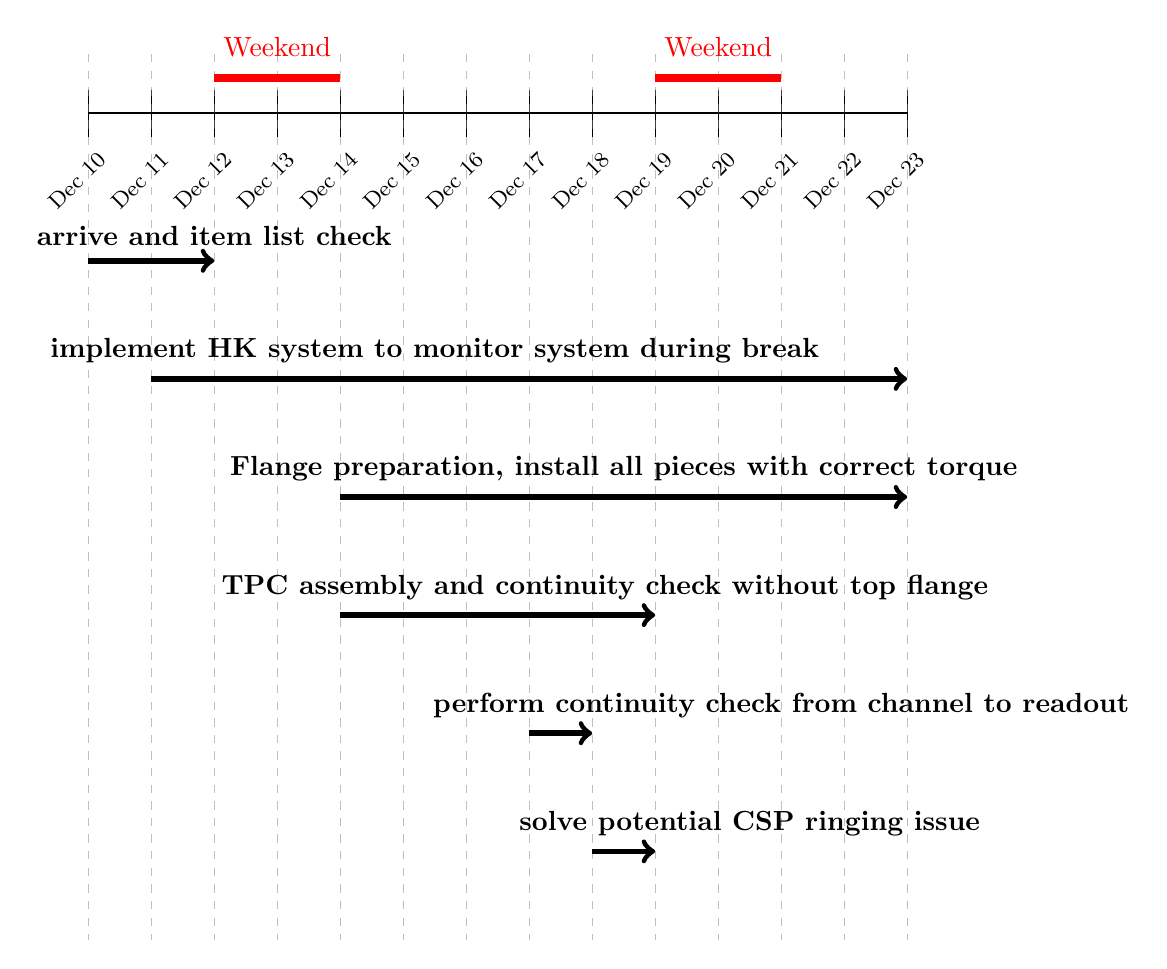
\begin{tikzpicture}[xscale=0.8, yscale=1.5]
    % Draw horizontal timeline
    \draw[thick] (0,0) -- (13,0);
    
    % Draw vertical date separators AND dashed lines
    \foreach \x/\date in {0/Dec 10, 1/Dec 11, 2/Dec 12, 3/Dec 13, 4/Dec 14, 5/Dec 15, 6/Dec 16, 7/Dec 17, 8/Dec 18, 9/Dec 19, 10/Dec 20, 11/Dec 21, 12/Dec 22, 13/Dec 23}
    {
        % Solid tick marks on timeline
        \draw (\x,0.2) -- (\x,-0.2);
        
        % Dashed vertical lines extending through entire chart
        \draw[dashed, gray, opacity=0.5] (\x,0.5) -- (\x,-7);
        
        % Date labels
        \node[below, rotate=45, anchor=north east, yshift=-2pt, xshift=2pt, font=\footnotesize] at (\x,-0.2) {\date};
    }
    
    % Weekend markers
    \draw[red, line width=3pt] (2,0.3) -- (4,0.3);
    \node[red, above] at (3,0.4) {Weekend};
    
    \draw[red, line width=3pt] (9,0.3) -- (11,0.3);
    \node[red, above] at (10,0.4) {Weekend};
    
    % task 1: arrival and item list check
    \draw[line width=2pt, ->] (0,-1.25) -- (2,-1.25);
    \node[above] at (2,-1.2) {\textbf{arrive and item list check}};
    
    % Task 2: implement HK system to monitor system during break
    \draw[line width=2pt, ->] (1,-2.25) -- (13,-2.25);
    \node[above] at (5.5,-2.2) {\textbf{implement HK system to monitor system during break}};
    
    % Task 3: flange preparation and install all pieces with correct torque
    \draw[line width=2pt, ->] (4,-3.25) -- (13,-3.25);
    \node[above] at (8.5,-3.2) {\textbf{Flange preparation, install all pieces with correct torque}};
    
    % Task 4: TPC assembly and continuity check without top flange
    \draw[line width=2pt, ->] (4,-4.25) -- (9,-4.25);
    \node[above] at (8.2,-4.2) {\textbf{TPC assembly and continuity check without top flange}};
    
    % Task 5: perform continuity check from channel to readout
    \draw[line width=2pt, ->] (7,-5.25) -- (8,-5.25);
    \node[above] at (11,-5.2) {\textbf{perform continuity check from channel to readout}};

    % Task 6: solve potential CSP ringing issue
    \draw[line width=2pt, ->] (8,-6.25) -- (9,-6.25);
    \node[above] at (10.5,-6.2) {\textbf{solve potential CSP ringing issue}};
    
\end{tikzpicture}
\caption{pGRAMS test bench at Osaka setup timeline}
\label{fig:Osaka_integration_schedule}
\end{figure}

% TODO: make Osaka pGRAMS backup chamber section

\begin{longtable}{|p{0.15\linewidth}|p{0.15\linewidth}|p{0.68\linewidth}|} 
\caption{pGRAMS Osaka bench Components list} \label{tab:Osaka_components} \\
\hline
\multicolumn{2}{|c|}{ARIOS chamber} & chamber body, CF12 gasket, CF12 gasket(backup), CF12 bolts and nuts(M8 70mm), CF12-CF10 adapter, CF10 bolts and nuts(5/16. 1.25), CF10 gasket, CF10 gasket(backup), CF10 flange, styrofoam \\
\hline
\endfirsthead

\multicolumn{3}{c}%
{{\bfseries \tablename\ \thetable{} -- continued from previous page}} \\
\hline
\multicolumn{2}{|c|}{ARIOS chamber (continued)} & \\
\hline
\endhead

\hline \multicolumn{3}{r}{{Continued on next page}} \\ \hline
\endfoot

\hline \hline
\endlastfoot

\multirow{10}{*}{CF10 air side} & CF4.5 flange & CF4.5 gasket, CF4.5 bolts (tapped hole), M8 25mm, CF4.5-CF4.5-CF4.5 tee, CF4.5 gasket, CF4.5 bolts and nuts, M8 50mm, CF4.5 DB25 flange, DB25 femail connectoe kit (for airside), DB25 RTD, MH ADC board v2, Molex connectors and socket, CF4.5 gasket, CF4.5 bolts and nuts, M8 50mm, CF4.5-CF4.5 valve, CF4.5 gasket, CF4.5 bolts and nuts, M8 50mm, ISO100 to CF4.5 adapter, ISO100 o-ring, ISO100 clamp, ISO100 hose, ISO100 o-ring, ISO100 clamp, ISO100 90-degree, ISO100 o-ring (to turbo), ISO100 clamp \\ 
\cline{2-3}
 & CF2.75 flange & CF2.75 gasket, CF2.75 bolts (tapped hole), M6 18mm, CF2.75-CF2.75-CF2.75 tee, CF2.75 gasket, CF2.75 bolts and nuts (LDS kit, 1/4-28, 1.25"), CF2.75 viewport, CF2.75 gasket, CF2.75 bolts and nuts (LDS kit, 1/4-28, 1.25"), CF2.75 to CF1.33 flange, CF1.33 gasket, CF1.33 bolts (tapped hole) 8-32 0.5", CF1.33 SHV 5kV feedthrough and cable \\ 
\cline{2-3}
 & CF1.33 \#1 & CF1.33 gasket, CF1.33 bolts (tapped hole) M4 12mm, CF1.33 blank \\ 
\cline{2-3}
 & CF1.33 \#2 & CF1.33 gasket, CF1.33 bolts (tapped hole) M4 12mm, CF1.33 blank \\ 
\cline{2-3}
 & CF1.33 \#3 & CF1.33 gasket, CF1.33 bolts (tapped hole) M4 12mm, CF1.33 - CF1.33 extension, CF1.33 gasket, CF1.33 bolts and nuts (LDS kit), CF1.33-CF1.33-CF1.33 tee, CF1.33 gasket, CF1.33 bolts and nuts (LDS kit), CF1.33 rupture disk, CF1.33 gasket, CF1.33 bolts and nuts (LDS kit), CF1.33 - KF25 adapter, KF25 o-ring and clamp, KF25 MKS gauge (new one), MKS readout cable \\ 
\cline{2-3}
 & CF1.33 \#4 & CF1.33 gasket, CF1.33 bolts (tapped hole) M4 12mm, CF1.33 - swagelok 3/8'' adapter (male), SS tube, 3/8" (long), swagelok 3/8'' ferrules and nut, swagelok 3/8'' valve (male-male), swagelok 3/8'' ferrules and nut, SS tube, 3/8" (short), swagelok 3/8''-1/4''-3/8'' tee (all males), swagelok 1/4'' ferrules and nut, SS tube, 1/4" (long), swagelok 1/4'' adapter (male-male), swagelok 1/4'' analog pressure gauge, swagelok 3/8'' ferrules and nut, SS tube, 3/8" (short), swagelok to NPT adapter (male-female), NPT passive relief valve (male) \\
\cline{2-3}
 & CF1.33 \#5 & 1/2 inch PTFE tube, CF1.33 gasket, CF1.33 bolts (tapped hole M4 12mm), swagelok 1/2'' ferrules and nut, CF1.33 vacuum-swagelok 1/2'' tubing (female), swagelok 1/2''-3/8'' adapter (male-male), swagelok 3/8'' ferrules and nut, SS tube, 3/8" (long), swagelok 3/8'' valve (male-male), swagelok 3/8'' ferrules and nut, SS tube, 3/8" (short), 1/2" VCR male to 3/8" swagelok adapter \\
\cline{2-3}
 & CF1.33 \#6 & CF1.33 gasket, CF1.33 bolts (tapped hole) M4 12mm, CF1.33 vacuum-swagelok 1/2'' tubing (female), swagelok 1/2'' ferrules and nut, swagelok 1/2''-3/8'' adapter (male-male), swagelok 3/8'' ferrules and nut, SS tube, 3/8" (long), swagelok 3/8'' valve (male-male) \\
\cline{2-3}
 & threaded holes & M8 eyeballs for lifting \\
\cline{2-3}
 & signal flange &  air side readout DB50 breakout boards, SMA cables, inner side DB50 adapter board, 4-40 vented screw, 3/8" long, DB37-DB37 signal adapter cable \\
\hline
\multirow{2}{*}{Vacuum side} & TPC mounting & M8 vented screws, 16 mm, M8 vented screws, 35 mm, C-clamps, 4.5 cm space, C-clamps, 3 cm space, M8 threaded rod, 25 cm, mounting disk, SS \\
\cline{2-3}
 & TPC & TPC body, CSP, SIPM preamp board, CSP power board, SMA cable for CSP power boards, SMA cable for SiPM boards, cryo-SMA cable for CSP power/SiPM, SMA extension adapter (female to female), SMA tee, PTFE TPC adapter top 1, PTFE TPC adapter top 2, PTFE TPC adapter bottom 1, PTFE TPC adapter bottom 2 \\
\hline
\multicolumn{2}{|l|}{vacuum pumps} & scroll pump, hose, clamps, turbo pump, turbo 24V power supply, turbo controller/RPi, RS485 to USB adapter, turbo power cable \\
\hline
\multicolumn{2}{|l|}{Tools etc} & tool box: socket wrench, hex kit, torque wrench, zip ties, dental floss, PTFE tape, Straps, screw drivers, Solder bench, cutter, scissors, adjustable wrenches, nitro gloves, \ac{PPE} \\
\hline
\end{longtable}

\begin{figure}
    \centering
    \includegraphics[width=1\linewidth]{fig/Osaka_pgrams.png}
    \noindent\raggedright Left picture shows the final outlook of the pGRAMS backup chamber at Osaka. All components were installed on the CF-12 flange and tightened with correct torque, pumped from the ISO100 hose by the HiPace 300 turbo pump. Right picture shows the inside of the chamber with TPC mounted on the stainless steel mounting disks. 
    \caption{pGRAMS test bench at Osaka setup}
    \label{fig:Osaka_chamber_setup}
\end{figure}

Fig.~\ref{fig:Osaka_chamber_setup} shows the final outlook of the pGRAMS backup chamber at Osaka. All components were installed on the CF-12 flange and tightened with correct torque, pumped from the ISO100 hose by the HiPace 300 turbo pump. Right picture shows the inside of the chamber with TPC mounted on the stainless steel mounting disks. After pumping, we have performed multiple leak checks with ethonol to ensure there is no leak point on the entire system.
This shows the capabilities of replicate a full pGRAMS system in a different location with a different team in a short amount of time, makes another advantage for liquid argon time projection chamber technology for a variety of applications for succesors to adapte.


\subsection{pGRAMS Flight Detector}
\label{chap:GRAMS:pGRAMS:detector}
\begin{figure}
    \centering
    \includegraphics[width=1\linewidth]{fig/pGRAMS_TPC_model_v2.png}
    \noindent\raggedright Left figure shows miniGRAMS TPC design demonstration. Top anode is constructed with a $ 330\ mm \times 330\ mm $ tile, and 12 groups of \ac{CSP}. Bottom cathode is constructed of 3 SiPM preamp boards which holds 3 cells each. Inside TPC there are PTFE sheet to separate each cells. Right figure shows miniGRAMS TPC schematic. Each field cage rings for TPC body is connected with a 100 M$\Omega$ resistor while anode mesh region is connected with a 400 M$\Omega$ resistor to provide desired E-field ratio between these two regions.
    \caption{MiniGRAMS \ac{LArTPC} detector design demonstration}
    \label{fig:minigrams}
\end{figure}
pGRAMS will make use of the ``MiniGRAMS'' LArTPC detector, which comprises a total of nine (9) optically isolated TPC cells, as shown in Fig.~\ref{fig:minigrams}, housed inside the cryostat with a custom flange. LArTPC is constructed with 
\begin{itemize}
    \item Top electron readout system that 180 of charge sensitive preamps(CSPs) connected to a 2D charge sensing tile to provide the electron drift x-y geometry information, which is powered by a serial of power board to distribute the power and signal and same time.
    \item serials of field shape rings embedded in four side PCB boards to provide the drift E-field.
    \item Anode and cathode mesh for field shaping and extract drifted electrons
    \item bottom 3x3 SiPM cells to readout the signal trigger light that is produced inside the active volume
\end{itemize}
See Fig.~\ref{fig:minigrams}, Left figure shows miniGRAMS TPC design demonstration. Top anode is constructed with a $ 330\ mm \times 330\ mm $ tile, and 12 groups of \ac{CSP}. Bottom cathode is constructed of 3 SiPM preamp boards which holds 3 cells each. Inside TPC there are PTFE sheet to separate each cells. Right figure shows miniGRAMS TPC schematic. Each field cage rings for TPC body is connected with a 100 M$\Omega$ resistor while anode mesh region is connected with a 400 M$\Omega$ resistor to provide desired E-field ratio between these two regions.

\noindent\textbf{Charge readout anode:} The charge collection tile has a geomatry of 33~cm$\times$33~cm which shares the same design concept as described in Section.~\ref{chap:GRAMS:pGRAMS:RandD:detector}. Its active area is 30~cm$\times$30~cm from the outer contour, while there will be no active area on the edges on each cell due to separation. Tile itslef comprises 96 strips on each direction (X and Y), spaced 2.6~mm apart, read out independently. Due to the cell separator, there will be 90 strips on each direction be active, which added to total 180 charge readout channels. Each strip is made of pixels connected along the given direction and inteplexed as shown in Fig.~\ref{fig:microGRAMS_RandD} (a), (b) and (c). Once the charge reached tile, it will induce both X and Y strips to let us grab the information of the hit location. Detailed design files of miniGRAMS tile are listed in appendix.~\ref{app:designs}.

\subsection{Data acquisition system (DAQ)}
\label{chap:GRAMS:pGRAMS:DAQ}
As system diagram of pGRAMS shown in Fig.~\ref{fig:system_diagram}, the \ac{DAQ} system is responsible for reading out the charge signals from the \ac{LArTPC} detector, digitizing them, and transmitting the data to the onboard computer for storage and analysis. The \ac{DAQ} system is designed to handle the high data rates generated by the TPC, while also being robust enough to operate in the harsh conditions of a balloon flight. After passing cryostats and vacuum jacket flanges, the amplified charge signals from the CSPs are feeded into a special shaper board designed by Columbia University to further shape the signals rising peak for better timing resolution. Then the shaped charge signals are sent to Neis DAQ crate that lives inside the sealed enclosure to get digitized and transmitted to the DAQ computer via PCIe. While at the same time TPC light signals will be sent to a shaper card lives in the same Nevis crate for further shaping and digitization. Light rigger will also be digitized and sent to DAQ computer via PCIe, and provide a trigger signal to \ac{TOF} system for further event mergers.

\noindent\textbf{Charge DAQ Nevis DAQ crate Mechanical assembly:} The system comprises a 9U crate with a custom backplane, a crate controller, a clock card, a transmitter module, a trigger board, and three ADC+FEM (Front End Module) cards responsible for digitization and data processing.  The crate is housed inside the sealed enclosure, due to the environment and thermal requirements. 

\noindent\textbf{Charge DAQ digitization and Data Handling:} The analog TPC data are received by each ADC+FEM card in groups of 64 channels. The ADC part of the card was designed by Brookhaven National Lab, while the digital data handling part was designed by Columbia University, Nevis Labs. Within each card, the analog signals are digitized within eight AD9222 octal-channel, 12-bit ADC chips from Analog Devices, Inc., providing sufficient dynamic range to accommodate both gamma-ray and antiparticle detection, with a power consumption of 100~mW/channel. Signals are digitized at 16~MHz, but only one in eight samples are kept in the digital handling part of the board, reducing the sampling rate to effectively 2~MHz. The 2~MHz sampling rate is optimized by taking into consideration the expected pulse shape provided by the convolution of the front-end electronics, the expected electric field response, and the O(1)~$\mu$s diffusion effects which govern charge drift within the liquid argon. Digital handling is provided by the FEM part of the card, which houses a Stratix III Altera FPGA. Data from all 64 wires are first rearranged from channel order to time order, and duplicated into two readout streams---one that supports continuous readout after loss compression, and another that allows for lossless compression and readout upon receiving an external trigger. Only the latter option was chosen for pGRAMS.

\noindent\textbf{Charge DAQ readout Configuration and Data Flow:} The crate controller provides system configuration and slow I/O communication with each board in the readout crate. The system is run on an independent, 16~MHz clock, distributed synchronously to all electronics cards via the backplane. The clock resets upon a software-initiated run-start and is tracked in terms of a configurable (nominally set to 100~us) frame size and a 2~MHz sample number keeping track of time within the frame. All ADC+FEM cards are synchronized to this common 16~MHz clock. The trigger board is responsible for receiving and issuing trigger signals, as well as distributing accepted triggers to the crate controller. The crate controller subsequently propagates them to the transmitter module. The latter initiates sequential readout of each ADC+FEM card beginning with a configurable readout window prior to the trigger time, $\Delta t$, and extending forward in time spanning a total of 3$\Delta t$. The configurable size of $\Delta t$ is governed by the maximum drift time and spans three or four frames. In order to reduce the amount of data being transmitted, the FPGA trims the three or four frames to span the exact readout window required, 100~$\mu$s before the trigger plus 200~$\mu$s after the trigger. Optionally, lossless compression (Huffman) can be applied, and, after processing by the FPGA, the data passes to the crate backplane dataway. A token-passing scheme is utilized to transfer data from each FEM board to the data transmitter module in a controlled way, whereby each FEM, in the order of closest to furthest away from the XMIT module, receives a token, transmits its data to the XMIT, and passes the token on to the next FEM in the sequence. Each FEM sends all data associated with a particular trigger number. This data transfer is relayed via the otherwise passive crate backplane, and is limited to 512~MB/s. In the transmitter module, the data is buffered temporarily and sent to the DAQ machine via PCIe.

\noindent\textbf{Light DAQ capture light trigger:} The Trigger Board has the ability to receive, via the crate controller, DAQ-issued (via software) calibration triggers, which are used explicitly for electronics and light calibration. The various input triggers can be independently pre-scaled, masked, and mixed together (OR or AND) to generate an event trigger to make sure we capture all the \ac{ROI}.

\noindent\textbf{Light DAQ Mechanical Assembly:} The nominal option for the pGRAMS SiPM readout makes use of custom readout electronics designed originally for the MicroBooNE LArTPC experiment, and is a complement to the charge readout system. Specifically, the light readout system can be housed together with the charge readout system in the same custom crate with a backplane distributing power and clock signals to a number of electronics boards:
\begin{enumerate}
    \item Crate Controller: responsible for configuration and control at run start, status readback and GPS timing readback. Also receives trigger from trigger board and issues readout command.
    \item Shaper board: Receives raw analog signals from SiPMs. Shapes signals with a ~60ns rise time. Shaped signals are driven differentially to the ADC+FEM via front panel cables.
    \item ADC+FEM board: Performs digitization and data packaging. The board supports up to 64 channels (only 1 will be needed for pGRAMS).
    \item Transmitter board (XMIT): Responsible for shipping the ADC+FEM data. The XMIT hardware supports two possible streams: triggered, or continuous.
    \item Trigger board: Receives SiPM triggers from the ADC+FEM board. The trigger board issues triggers via ethernet connection to the crate controller.
    \item Clock module: 16MHz precision clock responsible for providing timing through the backplane to all boards.
\end{enumerate}

\begin{figure}
    \centering
    \includegraphics[width=0.7\linewidth]{fig/ADC_FEM_SCHEM.png}
    \caption{NEVIS DAQ schematic}
    \label{fig:DAQ_schematic}
\end{figure}

The SiPM ADC+FEM and three shaper boards can sit in the same crate as the charge readout system described eariler, in which case no extra crate or controller, \ac{XMIT}, clock, trigger modules would be necessary. The Columbia light readout system therefore only requires 4 additional boards, in the form of 3 analog shaper boards (5V) and a single ADC+FEM board (12V/5V).

\noindent\textbf{Light DAQ Digitization and Data Handling:} The analog waveforms enter the SiPM shaper board via LEMO inputs and are 50-Ohm terminated at the shaper. The shaped signals (unipolar shaping, 60ns shaping time) are sent to the ADC+FEM board differentially via short front panel cables, and are digitized by the ADC at 64 MHz. The baseline of the receiver is set at ADC mid‐range, 2048. After digitization, the digitized raw pulse is delayed by d=4 64 MHz samples and subtracted from itself, giving DIFF(i) = rawpulse(i)‐rawpulse(id), where d is a parameter configurable by the run control. This sharpens the pulse by removing any low frequency noise and baseline shifts. The value of d depends on the signal shaping time, and can be adjusted in order to maximize signal to noise ratio. If rawpulse(i)‐rawpulse(i‐d) is negative, DIFF(i) is set to zero. The DIFF pulse (which is NOT recorded but only used for generating readout conditions and triggering) is discriminated to determine whether rawpulse(i) should be read out, as well as to form a trigger. For any enabled channel, there are two discriminators, Discr 0 and Discr 1. Each has an independently set threshold value. A two‐level discrimination is used. Discr 0 is the first level of discrimination and is a precondition for Discr 1 firing. Discr 0 has a very low threshold and is used to determine the timing of a pulse, thus avoiding slewing. A second level of discrimination is applied by Discr 1. Discr 1 typically has higher thresholds and is used to determine the actual readout of data and define timing windows for possible SiPM trigger generation. If the discriminators fire on a particular channel, a configurable number of 64MHz samples for that particular channel associated with the fired discriminators will be stored in the FEM channel FIFO. If a trigger, issued by the trigger board, intercepts the FEM delay memory, the SRAM discriminated data over four clock frames surrounding the trigger time will be read out. Assuming the nominal choice of 100 microseconds per clock frame, this means 400 microseconds of SiPM data for every triggered event. 

\textbf{Light DAQ Readout Configuration and Data Flow:} The overall readout system's internal communication and data flow is described earlier in the charge DAQ part. The transmitter module initiates controlled and sequential readout of all ADC+FEM cards in the crate. The SiPM ADC+FEM stores four clock frames' worth of data for each event, including the frame in which the trigger was received, one frame before it, and two frames after it. A token-passing scheme is utilized to transfer data from each FEM board to the data transmitter module in a controlled way, whereby each FEM, in the order of closest to furthest away from the XMIT module, receives a token, transmits its data to the XMIT, and passes the token on to the next FEM in the sequence. It is necessary for the SiPM ADC+FEM to sit farther from the XMIT module than the TPC ADC+FEMs.


\subsection{Cryostat and plumbing}
\label{chap:GRAMS:pGRAMS:cryostats}
As main medium for \ac{LArTPC} is natually liquid argon which required a cryogenic system to handle the cooling and maintain the liquid state. For pGRAMS flight, we designed a custom cryostat with a vacuum jacket to provide the thermal insulation. The cryostat inner vessel is made of aluminum to hold the miniGRAMS \ac{LArTPC} detector and \ac{LAr} inside. The outer vessel is also made of aluminum to provide vacuum insulation space between inner and outer vessel to minimize the convection heat transfer. Then there are multi-layer of sheets wrapped around the inner cryostats to further reduce the radiation heat transfer. For pGRAMS operation we made cthis cryostat's flange facing downward to reduce the material stacking on top of the detector active volume. See Fig.~\ref{fig:pGRAMS_cryostat}. Left \textbf{(a)} shows cryostat general view. miniGRAMS TPC is mounted inside the inner cryostat. There are kapton heaters installed outside of inner cryostat to help release the argon before descending. Right top \textbf{(b)} shows area that between inner cryostat and outer vacuum jacket. Green cylinders are G10 supporting rods for the purpose of low thermal conductance. Thin blue/red/yellow hoses are plumbing lines for fill/vent/\ac{LLD} respectively. middle-siezd yellow line shows safety rapture disk. Right bottom \textbf{(c)} shows bottom of the cryostat. center KF cross is used for plumbing, while each quadrant has a signal flange for charge and light readout, \ac{HK} sensors, detector power flange and high voltage flange.With this cryostat design, we could maintain the \ac{LAr} state for more than 24 hours without any extra cooling. This is sufficient for the pGRAMS flight that targetting on last for less then one day.
Detailed cryostat design files are listed in appendix.~\ref{app:designs}.

\begin{figure}
    \centering
    \includegraphics[width=1\linewidth]{fig/pGRAMS_cryostat.png}
    \noindent\raggedright \textbf{(a)} Left figure shows cryostat general view. miniGRAMS TPC is mounted inside the inner cryostat. There are kapton heaters installed outside of inner cryostat to help release the argon before descending. \textbf{(b)} Right top figure shows area that between inner cryostat and outer vacuum jacket. Green cylinders are G10 supporting rods for the purpose of low thermal conductance. Thin blue/red/yellow hoses are plumbing lines for fill/vent/\ac{LLD} respectively. middle-siezd yellow line shows safety rapture disk. \textbf{(c)} Right bottom figure shows bottom of the cryostat. center KF cross is used for plumbing, while each quadrant has a signal flange for charge and light readout, \ac{HK} sensors, detector power flange and high voltage flange.
    \caption{pGRAMS cryostat design demonstration.}
    \label{fig:pGRAMS_cryostat}
\end{figure}

We have also setup a full plumbing system to handle the \ac{LAr} filling, venting and \ac{LLD} monitoring. The detailed plumbing schematic is shown in Fig.~\ref{fig:plumbing_schematic}. There are multiple safety protection mechanisms installed to avoid any over pressure or vacuum inside the cryostat during flight. Detailed argon filling procedure to be determined.
% TODO: update the argon filling procedure

We have done a series of analysis including thermal analysis and structural analysis to ensure the cryostat and plumbing system could survive the harsh environment during balloon flight. The thermal analysis shows that with the multi-layer insulation and vacuum jacket design, the heat load to the inner cryostat could be reduced to less than 30 W. Structural analysis shows that both inner and outer cryostat could survive the 10g acceleration during parachute deployment. Detail analysis report could be found in appendix.~\ref{app:software}.

\begin{figure}
    \centering
    \includegraphics[width=1\linewidth]{fig/pGRAMS_plumbing.png}
    \noindent\raggedright All argon will go through customized designed and regenerated filter to reduce nritrogon, oxygen and water Impurities. A scroll pump and vacuum pump will be used to clean up the inside of cryostat. 
    \caption{pGRAMS cryostat plumbing schematic.}
    \label{fig:plumbing_schematic}
\end{figure}

\subsection{Flight Computer System}
\label{chap:GRAMS:pGRAMS:computer}
The flight computer system is limited with stratosphere compatibility, low power consumption and system performance. Some selection requirement listed as:
\begin{itemize}
    \item computer that sends telementry data and controls \ac{PDU} has to be stratosphere compatible with wide temperature range from $-60^\circ C$ to $ +50^\circ C $.
    \item computer that reads and writes \ac{DAQ} system data has to have enough storage space and high data writing speed to avoid data loss. While at the same time hardware level it needs two \ac{PCIe} slots as data transition port as mentioned in Section.~\ref{chap:GRAMS:pGRAMS:DAQ}.
    \item power of the computer has to be as low as possible to perform necessary tasks.
    \item operating system has to be linux based to be compatible with the \ac{DAQ} software and other devices we are developing.
    \item exntension of I/O ports have to be flexible to connect with various devices including USB, RS232, SPI etc.
\end{itemize}

After evaluating multiple options, we have selected two computers to be the flight computer system for pGRAMS. One is the hub computer (Versalogic DS-EPM-31 BayCat) \cite{versalogic_baycat} that is responsible for overall system control telementry data handling. The other is the DAQ computer (Versalogic VL-EPMe-51 Sabertooth) \cite{versalogic_sabertooth} that is responsible for data receiving from Nevis DAQ crate via PCIe and store to local SSD. Both computers are running ubuntu 22.04. 
As system diagram of pGRAMS shown in Fig.~\ref{fig:system_diagram}, hub computer is mainly in charge of communication and control, while DAQ computer is mainly in charge of data receiving and storage, details described below in Section.~\ref{chap:GRAMS:pGRAMS:computer:hub} and Section.~\ref{chap:GRAMS:pGRAMS:computer:daq}.

For the control system, pGRAMS decided to use the same framework that is being used and tested in the engineer flight \cite{Nakajima:2024fgx}. See software development at \cite{pGramsFC_2024}.

\subsubsection{Hub Computer}
\label{chap:GRAMS:pGRAMS:computer:hub}
As we separate flight computers into two parts, hub computer is mainly in charge of communication and control. It will handle the communication with ground station via iridium and starlink. All \ac{HK} data collected from various sensors will be packaged and sent to ground station periodically. While at the same time it will also receive command from ground station and distribute the command to corresponding devices including \ac{PDU}, DAQ computer and \ac{TOF} system. This makes our options of hub computer more flexible since it doesn't need to handle high data rate from \ac{DAQ} system. We have selected Versalogic DS-EPM-31 BayCat \cite{versalogic_baycat} as our hub computer which is also being used for another balloon experiment ComPair \cite{10.1117/12.2628811}. 
As system diagram of pGRAMS shown in Fig.~\ref{fig:system_diagram} and Table.~\ref{tab:hub_io_summary}, hub computer will take 1 ethernet from flight provide worldview's avionics \cite{worldviewspace2025} as the primary control interface. The second ethernet connection will be used to connect with DAQ computer for command and status exchange. We will extend defualt USB ports to 6, connect to \ac{HK} board, 2x 4-wire \ac{RTD} readout modules, 2x \ac{TOF} bias control board converters and 1 spare. The communication before hub computer and \ac{PDU} would be through SPI interface and a pair of power cable.

\begin{table}
\centering
\begin{tabular}{@{}p{3cm}p{10cm}@{}}
\toprule
\textbf{I/O Interface} & \textbf{Specifications} \\
\midrule
\textbf{USB} & Four USB 2.0 host ports and one USB 3.0 host port. \\
\addlinespace
\textbf{COM 1 / 2} & RS-232/422/485 selectable. 16C550 compatible. 460 Kbps. \\
\addlinespace
\textbf{Digital I/O} & Twenty-four TTL I/O lines (3.3V). Independently configurable. \\
\addlinespace
\textbf{I2C} & Single I2C interface (3.3V) \\
\addlinespace
\textbf{Audio} & Via DisplayPort and HDMI interfaces, or optional VL-ADR-01 audio interface. \\
\addlinespace
\textbf{Counter/Timers} & Three 8254 compatible Programmable Interval Timers (PITs). \\
\textbf{Mini PCIe Socket} & Full-length Mini PCIe socket. Supports Wi-Fi modems, GPS receivers, non-volatile flash data storage with auto-detect mSATA support, and other plug-in modules. \\
\addlinespace
\textbf{SPI Interface} & Supports SPI and SPX devices. Supports up to two SPX modules. \\
\bottomrule
\end{tabular}
\caption{hub computer I/O Interface Summary}
\label{tab:hub_io_summary}
\end{table}

\subsubsection{DAQ Computer}
\label{chap:GRAMS:pGRAMS:computer:daq}
As hub computer takes most of the interface part, DAQ computer is mainly in charge of data receiving and storage. It will receive data from Nevis DAQ crate via PCIe and store to local SSD. We have selected Versalogic VL-EPMe-51 Sabertooth \cite{versalogic_sabertooth} as our DAQ computer which has a PC-104 slot and support high speed data writing to local SSD. It provides the performance we need while only consumes a maximum 50W power.
 As system diagram of pGRAMS shown in Fig.~\ref{fig:system_diagram}, DAQ computer will take one ethernet from hub computer for command and status exchange. There are two \ac{PCIe} slots adapted from PC-104 that will be used to connect with Nevis DAQ crate for data receiving. The other ethernet will be used to connect to \ac{TOF} system front end board D (FEB/D) for data receiving. There is only one USB port that is used to connect to a analog discovery 3 device \cite{digilent_ad3} for receiving and distibuting \ac{pps} clock signal.


\subsection{pGRAMS Gondola}
\label{chap:GRAMS:pGRAMS:gondola}
\begin{figure}
    \centering
    \includegraphics[width=1\linewidth]{fig/pGRAMS_gondola.png}
    \noindent\raggedright These two figures show the pGRAMS gondola design demonstration from front and back side of view. Center tower holds the cryostat, vacuum jacket and \ac{TOF} system, made the main structure of the detector. Two TOF panels are placed on top of the tower to provide the timing and trigger information. Four side of the tower are used to hold the \ac{MPD} panels. The base plate are used to mount all the battery stacks, while four outer side gondola are used for hub computer box, PDU, sealed enclosure respectively. Four legs with casters are designed to attach to the bottom of the base plate to enable flexibility of the payload during integration while they will be removed when we are preparing for launching.
    \caption{pGRAMS gondola design demonstration}
    \label{fig:pGRAMS_gondola}
\end{figure}
For holding all the subsystems together, we have designed a custom gondola for pGRAMS flight. See Fig.~\ref{fig:pGRAMS_gondola}, These two figures show the pGRAMS gondola design demonstration from front and back side of view. Center tower holds the cryostat, vacuum jacket and \ac{TOF} system, made the main structure of the detector. Two TOF panels are placed on top of the tower to provide the timing and trigger information. Four side of the tower are used to hold the \ac{MPD} panels. The base plate are used to mount all the battery stacks, while four outer side gondola are used for hub computer box, PDU, sealed enclosure respectively. Four legs with casters are designed to attach to the bottom of the base plate to enable flexibility of the payload during integration while they will be removed when we are preparing for launching. The gondola design follows the requirement of the mass budeget mentioned in Table.~\ref{tab:pGRAMS_massbudget} to ensure we have our flight altitude target met.

\subsection{Power Distribution Unit (PDU)}
\label{chap:GRAMS:PDU}
The power distribution unit (PDU) is responsible for distributing power from the battery packs to various subsystems of the pGRAMS payload, including the flight computer system, \ac{DAQ} system, \ac{TOF} system, cryostat heaters, and other electronics. The PDU is designed to handle the high power requirements of the payload while also being robust enough to operate in the harsh conditions of a balloon flight. We have specific control on \ac{PDU} with each devices, while the hub computer will remain always ON since it is the control end of the \ac{PDU}. Detailed design see Fig.~\ref{fig:design_PDU}.